\section{Self Control}

\subsection{Principle}
This section discusses another organic approach to traffic control. The traffic control techniques in the previous chapter used a FTC with a fixed cycle time to ensure a synchronisation between different controllers. The self control (SC) by L\"ammer and Helbing \cite{laemmer07} instead relies on an optimization technique that decides every second what the best phase is, so that the least vehicles have to stop and wait. Interestingly enough this leads to green waves too. We will show that in the following paragraphs.

\subsection{Setup}

\begin{figure} [!htb]
	\centering
	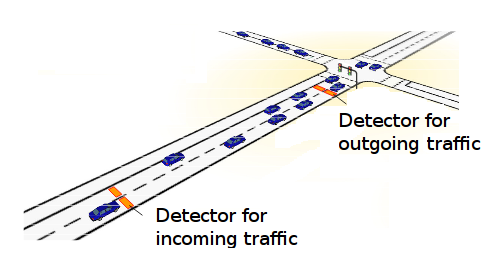
\includegraphics[scale=0.5]{pic/setup.png}
	\caption{Setup, L\"ammer (2009) \cite{laemmer09}}
	\label{img2}
\end{figure}

To make the self control work, there need to be detectors, traffic lights, controllers for the traffic lights and industrial computers. This setup does not need to be installed on every intersection, because the inherent organic nature of SC enables it to locally adapt to every traffic situation. The Detectors are used to determine the number and type of vehicles passing a lane to an intersection. They are placed at lanes which are incoming in relation to the intersection in question.There are detectors preferably far away from the intersection to detect incoming vehicles and detectors next to it to quantify outgoing vehicles.

\subsection{Anticipation, Optimisation and Stabilisation}

\begin{figure} [!htb]
	\centering
	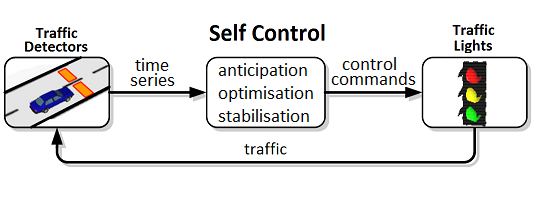
\includegraphics[scale=0.62]{pic/self_control_translation.png}
	\caption{Control loop, L\"ammer (2009) \cite{laemmer09}}
	\label{img1}
\end{figure}

%-----------------------Anticipation-------------------------
\subsubsection{Anticipation}
The information gathered by the detectors are needed to determine a series of predicted arriving times to the intersection and the number of already processed vehicles. After that a queueing model is used to calculate a required green time $\hat{g}_{i}$ to serve all not yet served vehicles $\hat{n}_{i}$. This is done for all traffic streams $i$ incoming into the intersection.

%-----------------------Optimisation-------------------------
\subsubsection{Optimisation}

\[
\sigma = max_{i} \{\pi_{i}\} 
\]

To decide which traffic stream gets the green light, the self control uses an optimisation technique. It assigns a priority $\pi_{i}$ to each traffic stream $i$ and the traffic stream with the highest priority $\sigma$  will get green light. $\pi_{i}$ is defined as.

\[\pi_{i} = 
\frac{\hat{n}_{i}}
{\tau^{pen}_{i,\sigma}+\tau_i+\hat{g}_{i}} 
%\quad with \quad 
%\tau^{pen}_{i,\sigma} = 
%\begin{cases}
%\phantom{-}x & \text{if } i \neq \sigma\\
%\phantom{-}0 & \text{if } i = \sigma
%\end{cases}
\]



\pi_{i}:   \phantom{-}   \text{priority of traffic stream} \\
\hat{n}_{i}:  \phantom{-}   \text{number of not served vehicles}\\
\tau_i:    \phantom{-}   \text{remaining set-up time}  \\
\tau^{pen}_{i,\sigma}:     \phantom{-}   \text{penalty cost for an extra set-up time}  \\
\hat{g}_{i}:   \phantom{-}   \text{required green time to serve all detected vehicles} \\


$\tau_i$ is the remaining set-up time. $\tau^{pen}_{i,\sigma}$ is the penalty cost for an extra set-up time, when i is not the current served traffic stream $\sigma$ i.e. the considered stream does not have green light. In case the considered traffic stream has currently green light ($i=\sigma$) the penalty $\tau^{pen}_{i,\sigma}$ is 0. That prevents constantly changing traffic lights.


The priority can be understood as a pressure acting on the intersection. The pressure of a traffic stream increases with the number of vehicles and takes the time to clear a lane into account. The intersection just needs to yield to the pressure and as a consequence minimises the cumulative waiting times for all vehicles. This principle has a psychological advantage too. It is easy to understand, so that traffic participants can predict how the SC behaves just by looking at the current traffic situation. Therefore it causes less frustration than other seemingly more chaotic organic approaches to traffic control.

When a bulk of vehicles are headed to an intersection controlled by SC they will likely get green light to minimize the waiting time. That is because the ratio of vehicles $\hat{n}_{i}$ and the required green time $\hat{g}_{i}$ will favor the traffic stream in question. By installing the SC on successive intersections green waves will naturally form without the need of individual controller communicating with each other. 


%-----------------------Stabilisation-------------------------
\subsubsection{Stabilisation}

\begin{figure} [!htb]
	\centering
	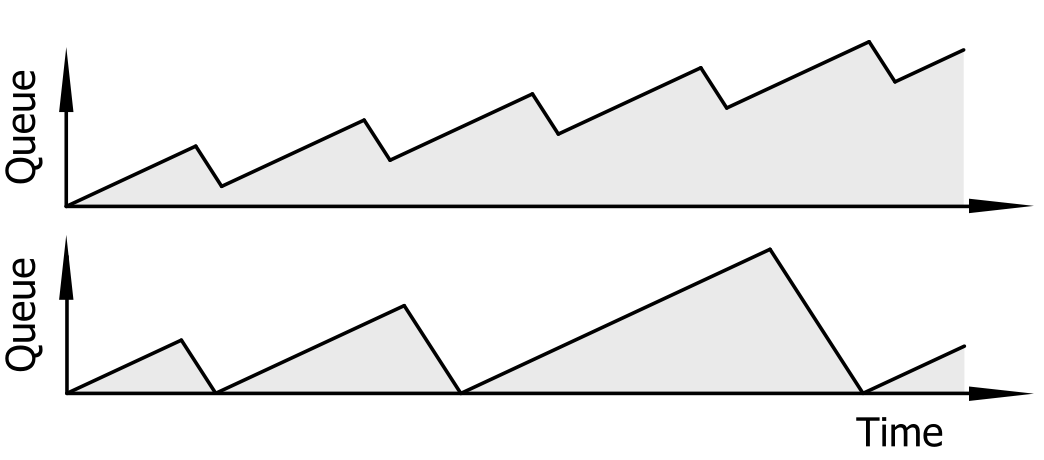
\includegraphics[scale=0.24]{pic/unstable.png}
	\caption{Examples of unstable waiting queues, L\"ammer (2009) \cite{stabilizing}}
	\label{img20}
\end{figure}

According to L\"ammer, a traffic light control is stable if the queue lengths will always stay finite \cite{laemmer08}. It is not hard to see that a traffic system in the real world demands stability, merely because of its inherent physical limitations. Fig. 8 shows examples of two unstable waiting queues. The intent of stabilisation is to prevent ever growing waiting queues which can easily occur with the current optimization. 

\[
\sigma  = 
\begin{cases}
\phantom{-}head \Omega & \text{if } \Omega \neq 0\\
\phantom{-}max_{i}\{\pi_{i}\} & \text{otherwise}
\end{cases}
\]

L\"ammer intruduces a local supervisory mechanism that observes the current traffic situation. When a critical number of waiting vehicles $\pi_{i}^{crit}$ is reached the corresponding traffic stream i is included into a priority set $\Omega$. The priority set $\Omega$ is organised as a FIFO list, meaning the first traffic stream i that is added to $\Omega$ is the first to be served. Whenever $\Omega$ is not empty, the head of the list gets priority. As soon as the queue is cleared ($n_i = 0$), or a maximal green time $g_{i}^{max}$ is reached, the stream i can finally get removed from $\Omega$. This dynamic is modeled by the equation seen above.

%--------------------Pedestrians, Cyclists and Public Transport---------------------
\subsection{Extension for Pedestrians, Cyclists and Public Transport}
Urban traffic does not exclusively consist of individual transport on the streets. Generally traffic lights in urban settings coordinate all types of traffic, such as pedestrians, cyclists and public transport. Fortunately, the presented method can be applied to all of them. All those types of traffic can be modeled as pressures with the use of queueing models.

The first adjustment that needs to be done are additional sensors to gather the required information of incoming traffic participants. Secondly the optimisation needs to be adjusted. The different types of traffic streams are weighted differently. For example it is reasonable to set the weights for trams as highest, the weight for buses as second highest and the weight for pedestrians as lowest.

Furthermore the weighting can depend on events. So might the weight of pedestrians be increased if a bus is waiting on the other side of the crosswalk at a bus stop. Or the weight of a tram can be set to zero if a bus from an airport is incoming. Another example would be an exponentially increasing weight for cars from small side streets, so that they get a chance to get green light.

%-----------------------Experiment-------------------------
\subsection{Experimental setup}

\begin{figure} [!htb]
	\centering
	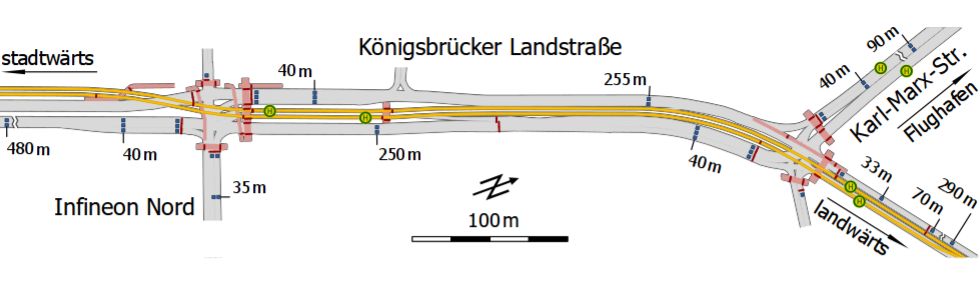
\includegraphics[scale=0.26]{pic/testing_area.png}
	\caption{Testing area in Dresden, L\"ammer (2015) \cite{laemmer15}}
	\label{testing_area}
\end{figure}

Before the SC was tested on a real road network it was tested in a simulation \cite{simulation} which suggested that the doability of the concept was given. 2015 L\"ammers SC was tested in Dresden \cite{laemmer15}. The setup was installed on two neighbouring intersections (K7
6 and K7) along K\"onigsbr\"ucker Landstra{\ss}e (Fig. \ref{testing_area}). The reason for L\"ammer to choose this area are that it is of reasonable small size but has a lot of complicated specifics in regard to traffic. 

The  K\"onigsbr\"ucker Landstra{\ss}e connects two districts of Dresden which results in dense traffic in the morning and the afternoon. In the busiest hour of the morning 900 Vehicles driving to and 500 are coming from the downtown area. In the afternoon these numbers are inverted. In Addition a tram and two bus lines a frequenting this area every 10 and 20 minutes. Furthermore there are traffic islands for pedestrians at the crosswalks.  

To evaluate the results to such an experiment it is important to know what kind of system was installed before the experiment took place. In this case a VS-PLUS (Version 6.2.5), as introduced in the state of the art section, was in use before. The V-PLUS utilised 12 induction loops to detect vehicles on the intersections in question.

The already installed hardware on K\"onigsbr\"ucker Landstra{\ss}e was not sufficient for the SC, so some hardware needed to be added.
On both intersection an independent industrial computer (Beckhoff CX2030) and a controller (C940VO) were installed to run the SC. Because the already implemented induction loops were too close to the intersections to work properly, 12 induction loops and 2 magnet sensors were added to the setup.

\begin{figure} [!htb]
	\centering
	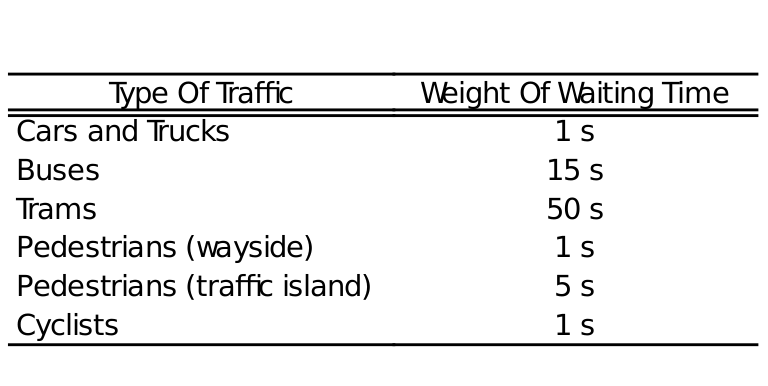
\includegraphics[scale=0.32]{pic/weighting.png}
	\caption{Weights, L\"ammer (2015) \cite{laemmer15}}
	\label{img66}
\end{figure}

As shown in Fig. \ref{img66} the weights for buses is 15 times higher than for cars and trucks and the weights for trams are even 50 times higher. Noticeable is that pedestrians get a 5 times higher weight than usually, if they are located on a traffic island.

Before and after the implementation of SC measurement data were taken. 20 persons measured waiting times and number of stops on 3 workdays each. Additionally 30 test drives were completed in both directions. Despite huge efforts to produce equal testing conditions, 10\% more vehicles passed K\"onigsbr\"ucker Landstra{\ss}e on the days after the implementation.

%-----------------------Results-------------------------
\subsection{Results}

Nonetheless SC has distinctly decreased the average waiting time for all groups of traffic participants. The diagrams in Fig. \ref{img44} to Fig. \ref{img42} are all build the same way. The grey bars to the left represent the average waiting time before the implementation of SC. The blue bars on the right side represent the average waiting time during the experiment. The width of the bars illustrate the amount of traffic.


\begin{figure} [!htb]
	\centering
	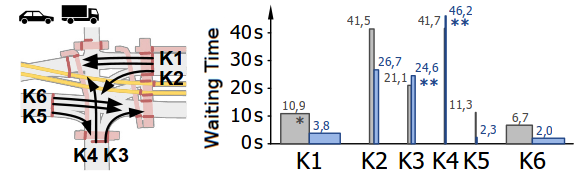
\includegraphics[scale=0.43]{pic/k6_waiting.png}
	\caption{ L\"ammer (2015) \cite{laemmer15}}
	\label{img44}

	\centering
	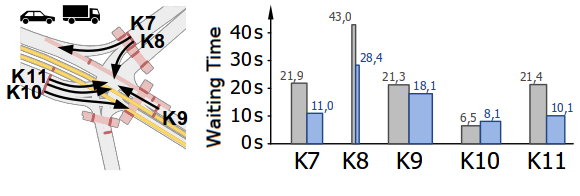
\includegraphics[scale=0.43]{pic/k7_waiting.png}
	\caption{L\"ammer (2015) \cite{laemmer15}}
	\label{img34}
\end{figure}

In Fig. \ref{img44} and Fig. \ref{img34} the average waiting times for cars and trucks can be seen. Noticeable 8 from 11 traffic streams reduced their waiting times perceptibly. But the data from K1 is not reliable because a electricity cut occurred during the testing phase with the VS-PLUS. The 3 that increased had already a low waiting time or contributed very little to the amount of traffic overall. According to L\"ammer, 2 of the increased average waiting times at K3 and K4 could be improved by simply adjusting the weight K4 and K5. That shows that the SC still needs a competent engineer to work properly and cannot completely control itself like the name SC suggests.

\begin{figure} [!htb]
	\centering
	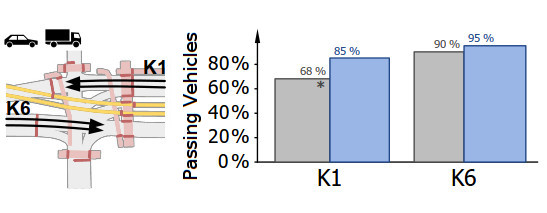
\includegraphics[scale=0.43]{pic/k6_durchfahrer.jpg}
	\caption{ L\"ammer (2015) \cite{laemmer15}}
	\label{img25}

	\centering
	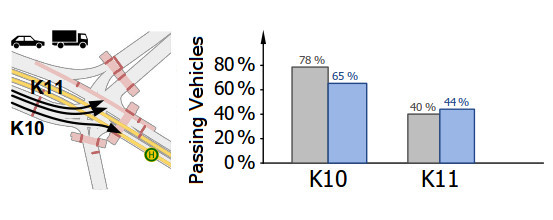
\includegraphics[scale=0.43]{pic/k7_durchfahrer.jpg}
	\caption{L\"ammer (2015) \cite{laemmer15}}
	\label{img26}
\end{figure}

Fig. \ref{img25} and Fig. \ref{img26} are showing the percentage of cars and trucks that could pass through the intersections without stopping once. Overall there could almost no improvement be observed by a increasing percentage average from 72,7\% to 73,4\%. 


\begin{figure} [!htb]
	\centering
	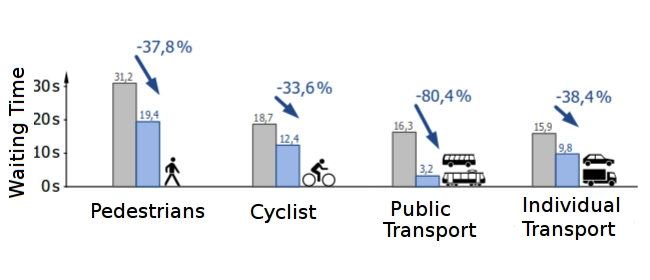
\includegraphics[scale=0.39]{pic/sc_results.jpeg}
	\caption{Average waiting time, L\"ammer (2015) \cite{laemmer15}}
	\label{img42}
\end{figure}

Fig. \ref{img42} shows the decreased overall average waiting time for every group of traffic participants. The huge decreased bar for public transport clearly reflects the high weight it got assigned. But even the pedestrians and cyclists, who got assigned the lowest weights, could decrease their average waiting times. It is important not to forget that these good results could be achieved despite the 10\% higher amount of traffic.
